\documentclass[conference,12pt]{IEEEtran}

\usepackage{hyperref}
\usepackage{graphicx, subfigure, amsmath} 
\usepackage[backend=biber,style=ieee]{biblatex}
\usepackage[section]{placeins}
\addbibresource{References/References.bib}
\interdisplaylinepenalty=2500

% correct bad hyphenation here
\hyphenation{}


\begin{document}
%
% paper title
\title{RoboTractor}
\author{
\IEEEauthorblockN{Jeremy Wright}
\IEEEauthorblockA{Arizona State University\\jlwrigh1@asu.edu}
\and
\IEEEauthorblockN{Arun Balaji Buduru}
\IEEEauthorblockA{Arizona State University\\abuduru@asu.edu}
\and
\IEEEauthorblockN{David Lucero}
\IEEEauthorblockA{Arizona State University\\dwlucero@asu.edu}
}
\maketitle


\begin{abstract}
    Here you need to describe the abstract of your project including (a) Problem statements, (b) project scope, (c) main tasks, and (d) schedule  *CRITICAL:  Do Not Use Symbols, Special Characters, or Math in Paper Title or Abstract. (Abstract)
\end{abstract}

\begin{IEEEkeywords}
    put indexing key words here that  (key words)
\end{IEEEkeywords}

\section{Introduction}
\IEEEPARstart{I}{n}  this section, describe:
\begin{enumerate}
    \item The problems to be addressed in this project.
    \item Why these problems are important?
    \item Applied technologies and solutions to address these problems.
    \item Expected outcomes of this projects.
    \item Project management plan (timeline, and group members, etc.)
\end{enumerate}
\section{System Models}

\subsection{System Model}
RoboTractor will leverage the Django Web framework \autocite{_django_2014}
, to realize the required
interfaces.  Figure~\ref{fig:softwarecomponents} describes the connection of
these components.  The combination of XMPP and REST in RoboTractor is
a demonstration of how to leverage the existing HTTP development environment
i.e. "the web of things" into a stateful protocol. HTTP is by design
stateless. XMPP on the other hand is a stateful streaming connection between two
clients. In this case the Tractor and a command server.  To achieve this mesh we
will leverage the Bidirectional-streams Over Synchronous HTTP standard
protocol \autocite{paterson_bidirectional-streams_2010}. BOSH provides
a standard mechanism to operate the streaming XMPP protocol efficiently over an
HTTP connection. This is essential for a scalable webservice. 
\subsection{Software}
\subsubsection{XMPP Server}
RoboTractor uses the ejabberd \autocite{_ejabberd} XMPP server as it provides an existing Python
interface, to integrate with the rest of our Python based ecosystem.
\subsubsection{REST Interface}
TastyPie provides REST \autocite{_toastdriven/django-tastypie_2014} by extending
the existing Django Models.
\subsubsection{BOSH Interchange}
Punjab is an Django plugin implementation of BOSH
\autocite{_twonds/punjab_2014}.  In addition to BOSH, this library also combines
th ejabberd Users with Django Users to provide a single authentication and
authorization framework. While this demo project will have a single user type,
this combination is critical to maintain proper use management and
least-privilege authorization.

\begin{figure}
\centering
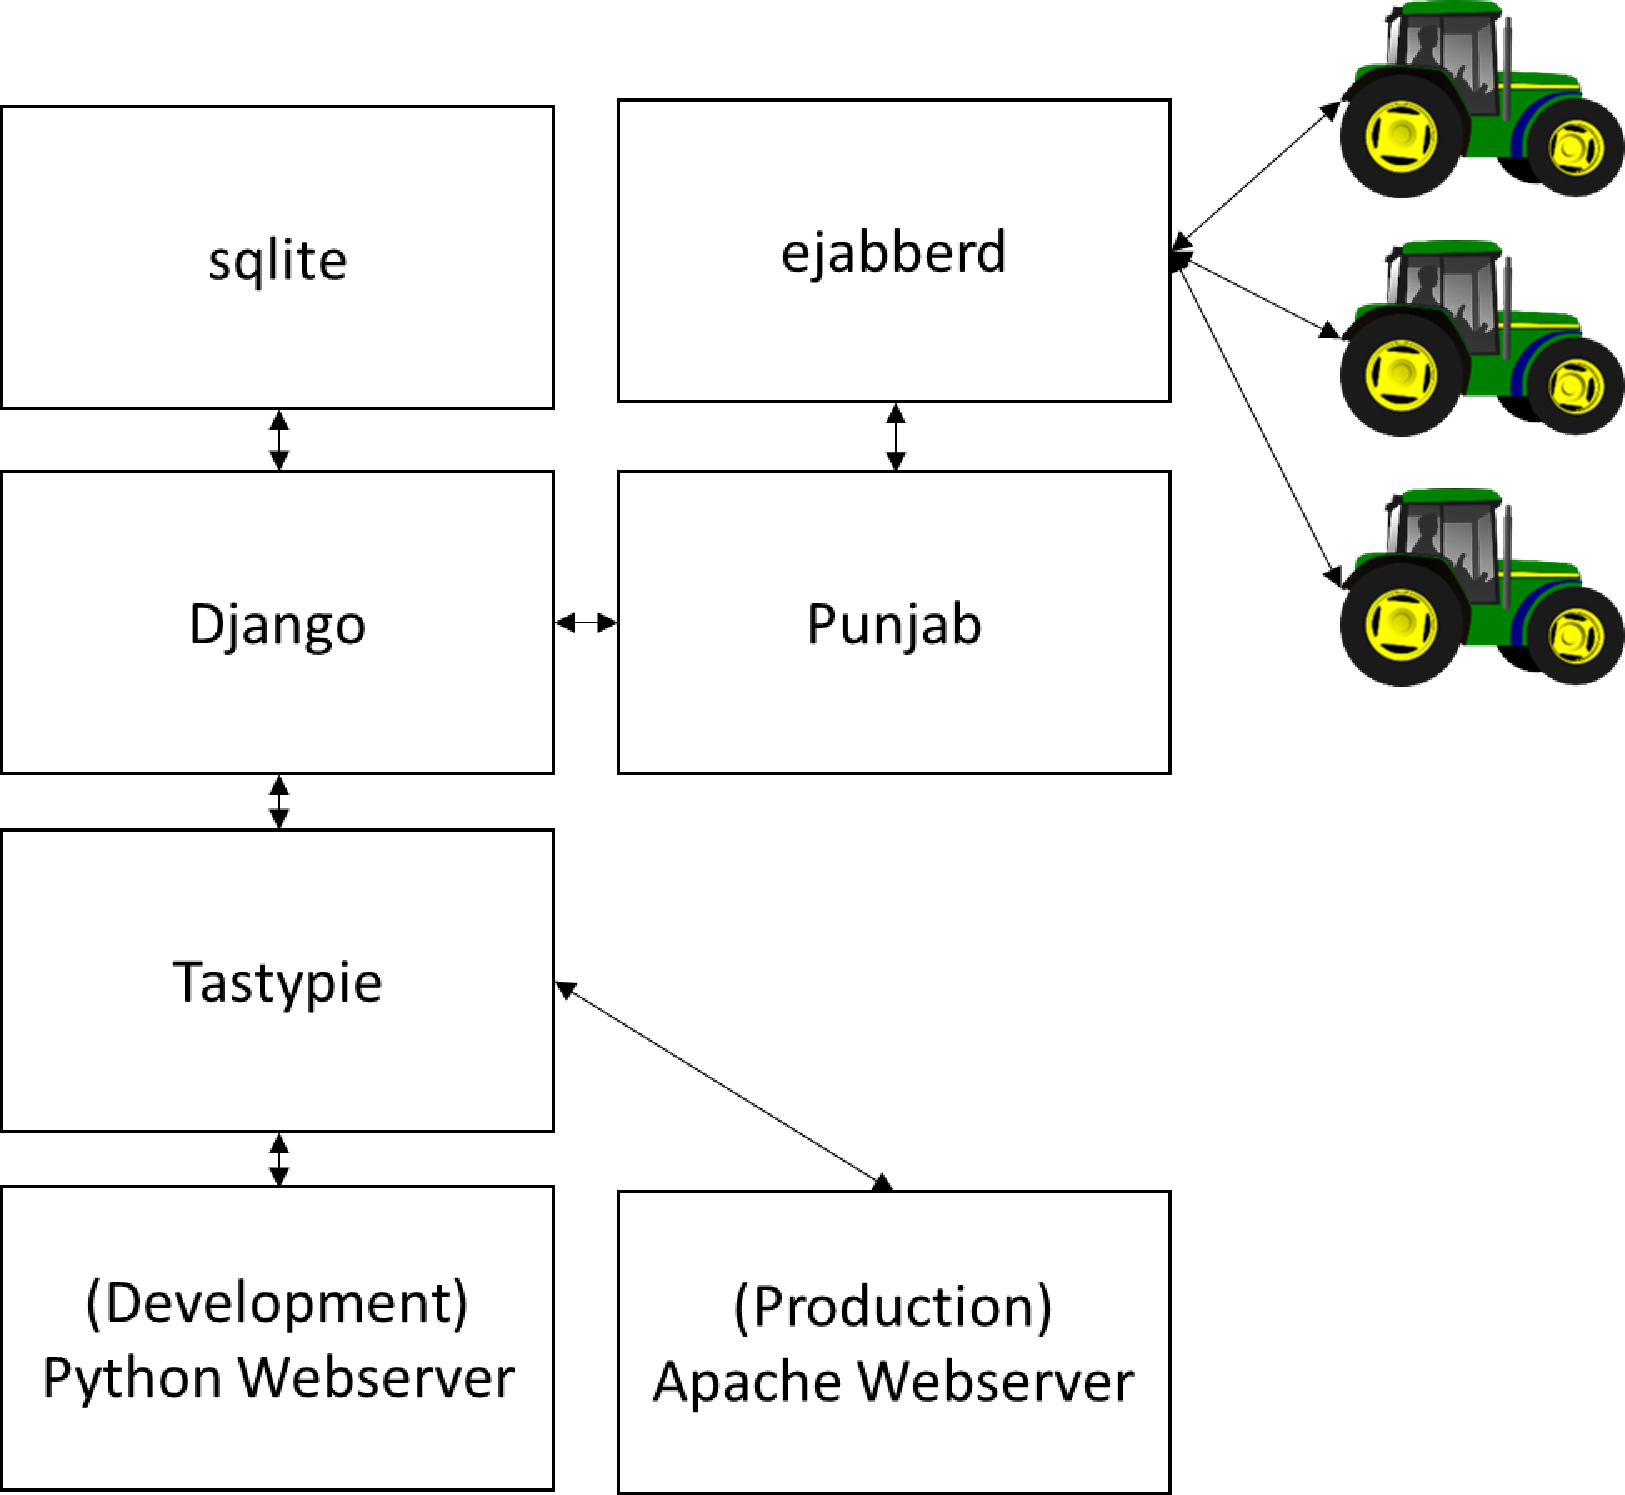
\includegraphics[width=0.4\textwidth]{SoftwareComponentBlockDiagram.pdf}
\caption{Software Component Block Diagram}
\label{fig:softwarecomponents}
\end{figure}

Describe needed software (applications, tools, APIs) to develop this project.
\subsection{Security Model (optional)}
This section is needed if the project is focusing on security. Describe attack source, attack goal, attach methods, and attack consequences. 
\section{Project Description}
Summarize the project description here.
\subsection{Project Overview}
Describe how many project tasks are proposed and what their relations (dependency) in the project. Use diagram is needed. Provide midterm and final goals of this project.
\subsection{Task 1 : title..}
Describe the proposed project task 1.
\subsection{Task 2: title..}
Describe the proposed project task 2.
\dots
\subsection{Task k: title..}
Describe the proposed project task k (if exists).
\subsection{Project Task Allocation}
Describe the workload for the group members and they responsibility for the proposed tasks. Use table if possible to highlight the proposed workload and allocations. Use percentle to indicate the workload and identify the project lead of this project.
\subsection{Deliverables}
Describe the expected outcomes of the projects: e.g., software packages, tools, algorithms, system designs, publishable materiasl (manuscripts, white papers, surveys, etc.).
\subsection{Project Timeline}
Describe the roadmap of the project. Use Gantt Chart if possible to highlight the project roadmap based on the project tasks. Provide the timeline of midterm and final goals of this project.
\section{Risk Management of the project}
Describe (a) what potential issues may prevent this project from being successful, (b) what mitigation strategies to prevent/mitigate the identified issues. A good project design should consider what if a task fails. How likely (low, medium, high), the proposed tasks may fail. Are there alternates/makeup/get-arround approaches available? Better use  a table to highlight the risks and corresponding mitigation strategy.

\section{Conclusion}
(a) summarize the project proposal, (b) Describe potential future work (or applications) that can be built based on the proposed work. 
\section{Acknowledgment }
Put sponsor/mentor/assistance acknowledgments on developing this project proposal.

Reference is very important in your report. Please highlight where you have
referred technical terms and solutions in the content. Following the IEEE
citation format and provide a complete citation for each reference. The template
will number citations consecutively within brackets [1]. The sentence
punctuation follows the bracket [2]. Refer simply to the reference number, as in
[3]—do not use “Ref. [3]” or “reference [3]” except at the beginning of
a sentence: “Reference [3] was the first ...” Here are a few examples.    \autocite{huang_ipv6_2014}
\printbibliography

    \end{document}


